\subsection{Database identification}
\label{sse:database}

The computation of visual information (e.g. keypoints features) needed
for image identification can be done offline and stored in a database.
For each image model we would like to identify in the current image, a
specific database item is created. Several items can also mixed
together to allow the identification of multiple images.

Figure~\ref{fig:ident_database} illustrates the structure of the database identification module:

\begin{figure}[H]
\centering
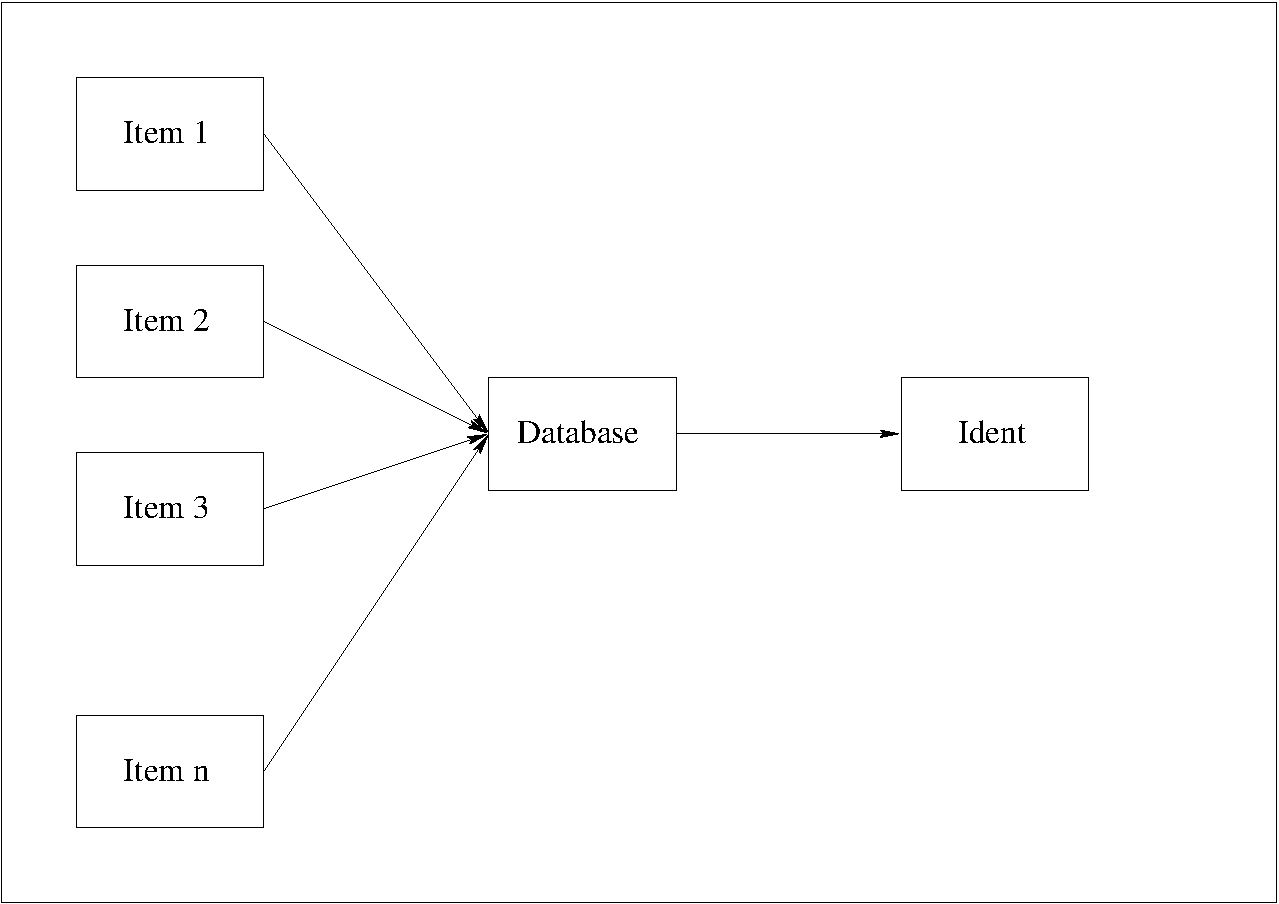
\includegraphics[width=0.75\textwidth]{vision/figures/ident_database} 
\caption{Structure of the database identification module.}
\label{fig:ident_database}
\end{figure}

\subsubsection{The {\tt Rox\_Ident\_Database\_SE3} object}
A \lstinline$Rox_Ident_Database_SE3$ object is a pointer to the opaque structure \lstinline$Rox_Ident_Database_SE3_Struct$: 

\begin{lstlisting}
typedef struct Rox_Ident_Database_SE3_Struct * Rox_Ident_Database_SE3
\end{lstlisting}

\subsubsection{Creating/Deleting a {\tt Rox\_Ident\_Database\_SE3}}

\noindent One database item is associated to one template. A Rox\_Ident\_Database may be considered as a collection of such database items. The database identification module is able to identify several templates simultaneously. Current library is optimized to run on up to 150 simultaneous templates. User can ask the module to detect all possible templates in the same current image or to detect only the most visible template (among the templates in the database). Speed degrades with the number of templates to track simultaneously and quality degrades with the number of templates in the database. It is possible to create several Rox\_Ident\_Database objects in the same program.\\

\noindent The rox\_ident\_database object shall be created before any call to other functions using it :

\begin{lstlisting}
Rox_Error rox_ident_database_se3_new (Rox_Ident_Database_SE3 *ident, Rox_Uint max_templates_simultaneous);
\end{lstlisting}

\noindent This function creates a new empty database object.

\begin{lstlisting}
Rox_Error rox_ident_database_se3_del (Rox_Ident_Database_SE3 *ident);
\end{lstlisting}

This function deletes the object. Shall be called when you do not need this database object anymore.

\subsubsection{Main functions related to {\tt Rox\_Ident\_Database\_SE3}}

% \begin{lstlisting}
% Rox_Bool rox_ident_database_add_template(Rox_Ident_Database
% obj, Rox_Char * pathtodb, Rox_Uint template_height, Rox_Uint template_width)
% \end{lstlisting}

% \noindent This function adds a template database file to the Rox\_Ident\_Database object. Please take care not to add several times the same database file. Template dimensions (template\_height and template\_width) are the dimensions of
% the reduced image to be used for further tracking process. Each time you add a
% template, an internal counter is incremented. The value of this counter is used
% as a unique ID for this template. Thus the template ID is a number between
% 0 and N-1 (N being the number of added templates).

\noindent The following function shall be called to enable
identification and prepare internal structures for optimized
execution:
\begin{lstlisting}
Rox_Error rox_ident_database_se3_set_database (Rox_Ident_Database_SE3 ident, Rox_Database db);
\end{lstlisting}

\noindent The following function execute identification process on the
image contained in the camera object. Uses all the templates added and
compiled before the call to this function. Once a template is found,
an internal flag is set and it will be ignored in further calls to
rox\_ident\_database\_process.
\begin{lstlisting}
Rox_Error rox_ident_database_se3_make (Rox_Ident_Database_SE3 ident, Rox_Camera camera);
\end{lstlisting}

\noindent To get the identification result for a given template ID use the following function: 

\begin{lstlisting}
Rox_Error rox_ident_database_se3_getresult (Rox_Uint *is_identified, Rox_MatSE3 pose, Rox_Ident_Database_SE3 ident, Rox_Uint id); 
\end{lstlisting}

\subsubsection{Creation of database items}

\noindent First, retrieve an image of your template without any perspective distortion. The biggest the image is, the better the detection will perform after database creation. However, if the image is too big the database file will be large and long to create. Ideally, the template size should be close to the image that will be viewed by the camera. The template image shall not contain large textureless regions and shall contain visual information everywhere. Please keep both files in a directory as they will be necessary for identification process.

The programmer can create its own database items by using the following function:
\begin{lstlisting}
Rox_Error rox_database_item_learn_template (Rox_Database_Item item, Rox_Image template); 
\end{lstlisting}

A database item can be saved on disk (use the extension ``.rdi'' for database items) using the following function:
\begin{lstlisting}
Rox_Error rox_database_item_save (Rox_Char *filename, Rox_Database_Item item);
\end{lstlisting}
A database item can be loaded using the following function:
\begin{lstlisting}
Rox_Error rox_database_item_load (Rox_Database_Item item, Rox_Char *filename);
\end{lstlisting}

%The programmer can create its own database item (extension .rdb) by using the following function:
%\begin{lstlisting}
%Rox_Bool rox_ident_database_create(const char *rdb_filename, Rox_Image image)
%\end{lstlisting}

\subsubsection{Creation of a database}

\noindent A database object shall be created using the following function:

\begin{lstlisting}
Rox_Error rox_database_new (Rox_Database *db));
\end{lstlisting}

\noindent This function creates a new empty database object.

The following function deletes the object.

\begin{lstlisting}
Rox_Error rox_database_del (Rox_Database *db); 
\end{lstlisting}
Shall be called when you do not need this database object anymore.

A database item can be added to the database using the following function:

\begin{lstlisting}
Rox_Error rox_database_add_item (Rox_Database database, Rox_Database_Item item, Rox_Real sizx, Rox_Real sizy);
\end{lstlisting}

After adding several items to the database, they can be fused in the database using the following function:

\begin{lstlisting}
Rox_Error rox_database_compile (Rox_Database database);
\end{lstlisting}

The resulting database can be saved on disk (use the extension ``.rdb'' for databases) using the following function:

\begin{lstlisting}
Rox_Error rox_database_save (char *filename, Rox_Database database);
\end{lstlisting}

and loaded from disk using the following function:

\begin{lstlisting}
Rox_Error rox_database_load (Rox_Database db, char *filename);
\end{lstlisting}

For client/server applications the user can serialise a database using the following function:
\begin{lstlisting}
Rox_Error rox_database_serialize (char *buffer, Rox_Database db);
\end{lstlisting}
and after sending it through the network, the user can deserialise it using the following function:
\begin{lstlisting}
Rox_Error rox_database_deserialize (Rox_Database db, char *buffer);
\end{lstlisting}

\subsubsection{Identification using database features directly}

In some applications, like cloud client/server applications, it is useful to store and use directly database features for the identifications. The features are stored in a Rox\_Database\_Features object. 

The programmer can use the following function to create database features:
\begin{lstlisting}
Rox_Error rox_database_features_new (Rox_Database_Features *features);
\end{lstlisting}

The Rox\_Database\_Features object can be deleted using the following function:
\begin{lstlisting}
Rox_Error rox_database_features_del (Rox_Database_Features *features);
\end{lstlisting}

The reference image can be therefore identified using the database features:
\begin{lstlisting}
Rox_Error rox_ident_database_se3_make_features (Rox_Ident_Database_SE3 ident, Rox_Database_Features features, Rox_Matrix calib_camera);
\end{lstlisting}


In the first case, the programmer can also serialize/deserialize the information in the Rox\_Database\_Features object in order to be sent through a network socket: 
\begin{lstlisting}
Rox_Error rox_database_features_serialize (Rox_Char *buffer, Rox_Database_Features features);
\end{lstlisting}

\begin{lstlisting}
Rox_Error rox_database_features_deserialize (Rox_Database_Features features, Rox_Char *buffer);
\end{lstlisting}

In the second case, the file containing the database features can be
created using the following function:
\begin{lstlisting}
Rox_Error rox_database_features_save (Rox_Char *filename, Rox_Database_Features features);
\end{lstlisting}
The file can be loaded using the following function:
\begin{lstlisting}
Rox_Error rox_database_features_load (Rox_Database_Features features, Rox_Char *filename);
\end{lstlisting}

See the example ``rox\_example\_identification\_database\_cloud.c'' for an example of use.
